 本章では最終成果発表で記入してもらった評価シートの集計結果とコメントを参考にして今後の改善点を記述する。
 評価シートの評価項目は「発表技術」と「発表内容」の2つと「発表内容」の細部に「複雑性にちての説明の評価」、「カウンティングについての説明の評価」の2つ合わせて計4つ用意した。そして、それぞれについて1(非常に悪い)から10(非常に優秀)までの間で評価点を記入する欄、それぞれについてのコメント(評価理由)やアドバイスを記入する欄をそれぞれ用意した。
\bunseki{葛西隼人}
\section{最終成果発表}
\subsection{評価点数の集計}
最終成果発表で記入してもらった評価シートは計50枚だった。シートを記入した人の所属の分布は表\ref{tab:dist2} のようになった。

\begin{table}[htb]
  \begin{center}
    \caption{評価人数集計}
    \begin{tabular}{|c|c|c|} \hline 
      所属 & 学年 & 人数  \\ \hline \hline
      教員 &  & 7  \\
      一般 &  & 8 \\
      学生 & 院2年 & 0 \\
     学生 & 院1年 & 0 \\
             & 学部4年 & 0 \\
       & 学部3年 & 31 \\
             & 学部2年 & 2 \\
             & 学部1年 & 2 \\ \hline \hline
      合計 &  & 50 \\ \hline
    \end{tabular}
    \label{tab:dist2}
  \end{center}
\end{table}

中間発表では一般の評価人数が0人だったが、今回は函館市内の高校生が来ていたため一般の評価人数は増えて8人だった。学生と教員に関しては学部4年が0人となった代わりに、学部1年が0人となっていた点以外は中間発表とほとんど差異のない構成人数であった。次はそれぞれの評価項目についての平均点を表\ref{tab:point2}に記す。
\begin{table}[H]
\begin{center}
\caption{評価点数集計}
\begin{tabular}{|c|c|c|c|c|c|} \hline
  所属 & 学年 & 発表技術 & 発表内容 & 複雑性説明 & カウンティング説明  \\ \hline \hline
  教員 &        & 7.42 & 7.14 & 7.14 & 6.71 \\ 
  一般 &        & 7.38 & 7 & 6.12 & 6.75 \\
  学生 &        & 7 & 7.2 & 6.66 & 7.02 \\
         & 学部1,2年 & 6.5 & 6.25 & 6.5 & 6.5 \\
         & 学部3年 & 6.87 & 7.39 & 6.7 & 7.26 \\ \hline \hline
  全体 &        & 7 & 7.2 & 6.66 & 7.02 \\ \hline
\end{tabular}
\label{tab:point2}
\end{center}
\end{table}

全体の平均は「発表技術」については7点、「発表内容」については7.2点、「複雑性説明」については6.66点、「カウンティング説明」については7.02点となった。中間発表と最終成果発表で「発表技術」のみ比較を行う。中間発表では6.69点、最終成果発表では7点となった。点数のみの比較でも0.31点高くなっている。これは中間発表からの技術改善が見られていると考えられる。「発表内容」については中間発表と異なるので比較は行わない。次に、それぞれの結果を図\ref{gizyutu2}、図\ref{naiyou2}、図\ref{hukuzatusei}、図\ref{counting}に示す。

\begin{figure}[h]
 \begin{tabular}{cc}
  \begin{minipage}[h]{0.45\hsize}
  \centering
 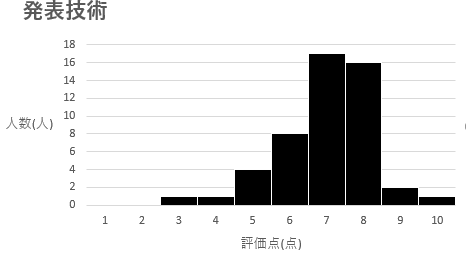
\includegraphics[width=0.7\linewidth]{./figure/gizyutu2.jpg}
\caption{発表技術の評価グラフ}
\label{gizyutu2}
 \end{minipage} &

\begin{minipage}[h]{0.45\hsize}
  \centering
 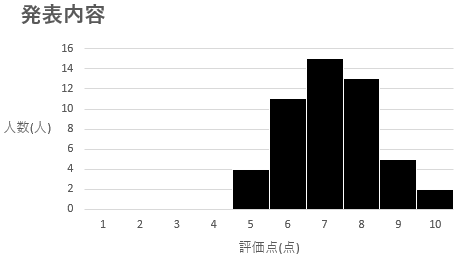
\includegraphics[width=0.7\linewidth]{./figure/naiyou2.jpg}
 \caption{発表内容の評価グラフ}
\label{naiyou2}
\end{minipage} 
\end{tabular}
\end{figure}

\begin{figure}[h]
 \begin{tabular}{cc}
  \begin{minipage}[h]{0.45\hsize}
  \centering
 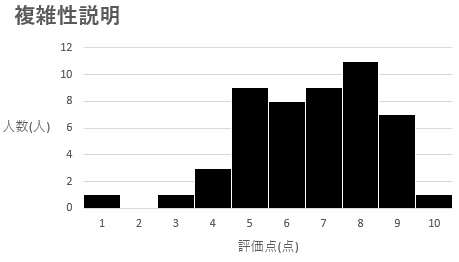
\includegraphics[width=0.7\linewidth]{./figure/hukuzatusei.jpg}
\caption{複雑性説明の評価グラフ}
\label{hukuzatusei}
 \end{minipage} &

\begin{minipage}[h]{0.45\hsize}
  \centering
 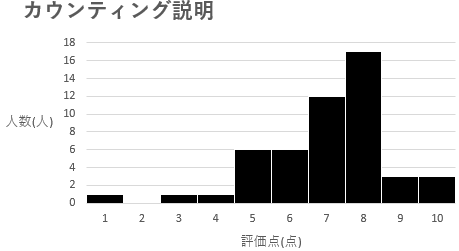
\includegraphics[width=0.7\linewidth]{./figure/counting.jpg}
 \caption{カウンティング説明の評価グラフ}
\label{counting}
\end{minipage} 
\end{tabular}
\end{figure}

「発表技術」と「発表内容」については評価点が共に7、8点と高い評価点が多かった。そして、「発表内容」に関しては最も低くても5点と全体的には評価はまとまっていたが、他のグラフは1,3
点など低い点数があり全体的な評価は散らばっていた結果となった。「複雑性説明」では5~8点の間にヒストグラムが集中していて理解度に差あることがわかった。

また、「発表技術」と「発表内容」の評価点数の相関係数は0.73となった。これは強い正の相関があり、2つの評価項目がかなり関連してると言える数値である。次にコメントについて解析する。
\bunseki{葛西隼人}

\subsection{コメント解析と改善点}
まず、「発表技術」について、肯定的なコメントと否定的なコメントに分けて並べる。

肯定的なコメント
\begin{itemize}
\item アニメーションがついてて見やすいスライドだと思った
\item アジェンダがあり、長いプレゼンがわかりやすかった
\item スライドの内容はよく整理されておりわかりやすかったです
\end{itemize}

否定的なコメント
\begin{itemize}
\item 発表場所が悪かったのもあり声がきこえないところがあった
\item 発表者が原稿を読んでいる感じがしたのが残念だった
\item 発表が単調で何が大事なポイントが分かりづらかった
\end{itemize}

スライド構成については評価するコメントはあったが、声が小さい、スライドの文字ばかり見ているとの発表者の技術面についての否定的な意見が多かった。そして発表の時間配分が他のプロジェクトと異なっていたため発表を全て聞けなかった人が少しいた。次に、「発表内容」についても同様に、肯定的なコメントと否定的なコメントに分けて並べる。

肯定的なコメント
\begin{itemize}
\item 仮説・実験・検証が適切に行われていた
\item 実験・検証が多く、説得力をもたせている
\item プロジェクト目標の設定が明確であった
\item 人間が使うことも含めた戦略の考察が面白いと思った
\end{itemize}

否定的なコメント
\begin{itemize}
\item エラー率は単純に複雑性から出すのではなく、似た状況がある時エラーするほうが正確なデータが出そうだと思った。
\item ポスターにもスライドにもチームとしてどう取り組んだのか全く示されていないのは、プロジェクト学習の発表として不十分に思えます
\end{itemize}

そして要望としてのあったコメントをいくつかあったので記述する。
\begin{itemize}
\item 勝率を100パーセントにしてほしい
\item 他のプロジェクトの発表もあるので、時間配分は考えてほしい
\end{itemize}

中間発表では、用語の説明が足りないというコメントが多く見受けられたが、最終成果発表ではカウンティングと複雑性の両方でわかりやすいというコメントがあった。今回の発表を通して得られた発表での留意点を以下に記述する。
\begin{itemize}
\item スライドは色を用いて見やすくする
\item 太線や下線などの重要な箇所を視覚的に理解できるようにする
\item 発表者は声は大きく、はっきり聞き取りやすく来ている人に目を向ける
\item 用語の説明を入れる、構成はアジェンダを用いてわかりやすくする
\end{itemize}

本プロジェクトでの中間発表と最終成果発表は今後の研究活動にも参考になる点が数多くあり非常に有益なものであった。
\bunseki{葛西隼人}